\documentclass[10pt, a4paper, twoside]{article}
\usepackage[T1]{fontenc}
\usepackage[utf8]{inputenc}
\usepackage[brazilian]{babel}
\usepackage{float}
\usepackage{booktabs}
\usepackage{graphicx, subcaption} 
    \graphicspath{{../figuras/}}

\usepackage{listings}
    \lstset{inputpath={listings/}}

\usepackage{tikz}
    \usetikzlibrary{positioning, arrows, arrows.meta, shapes.geometric}

\usepackage{color}

\usepackage{amsmath, amsthm, amssymb}
  \usepackage{stackengine}
\usepackage{scalerel}

\newcommand\dangersign[1][2ex]{%
  \renewcommand\stacktype{L}%
  \scaleto{\stackon[1.3pt]{\color{red}$\triangle$}{\tiny\bfseries !}}{#1}%
}

\newenvironment{remark}{\par\vspace{10pt}\small % Vertical white space above the remark and smaller font size
  \begin{list}{}{
    \leftmargin=35pt % Indentation on the left
    \rightmargin=25pt
  }\item\ignorespaces % Indentation on the right
  \makebox[-2.5pt]{%
    \begin{tikzpicture}[overlay]
      \node[inner sep=2pt,outer sep=0pt] at 
      (-15pt, 0pt)
      {\dangersign[3.5ex]};
    \end{tikzpicture}
  }
  \advance\baselineskip -1pt}{\end{list}\vskip5pt%
} %


%-----------------
%	THEOREM STYLES
%-----------------
\definecolor{azulunb}{cmyk}{1, 0.65, 0, 0.35}
\definecolor{verdeunb}{cmyk}{ 1, 0, 1, 0.2}

% Boxed/framed environments
\newtheoremstyle{bluenumbox}% Theorem style name
	{0pt}% Space above
	{0pt}% Space below
	{\normalfont}% Body font
	{}% Indent amount
	{\small\bf\sffamily\color{azulunb}}% Theorem head font
	{\;}% Punctuation after theorem head
	{0.25em}% Space after theorem head
	{\small\sffamily\color{azulunb}\thmname{#1}\nobreakspace\thmnumber{#2}\thmnote{\nobreakspace\sffamily\bfseries\color{black}---\nobreakspace#3.}} 
	% Optional theorem note

\newtheoremstyle{blacknumex}% Theorem style name
	{5pt}% Space above
	{5pt}% Space below
	{\normalfont}% Body font
	{} % Indent amount
	{\small\bf\sffamily\color{verdeunb}}% Theorem head font
	{\;}% Punctuation after theorem head
	{0.25em}% Space after theorem head
	{\small\sffamily{\tiny\ensuremath{\blacksquare}}%
		\nobreakspace\thmname{#1}\nobreakspace
		\thmnumber{#2}% Theorem text (e.g. Theorem 2.1)
		\thmnote{\nobreakspace\sffamily\bfseries---\nobreakspace#3.}
	}% Optional theorem note
\makeatother

% Defines the theorem text style for each type of theorem to one of the two styles above

\theoremstyle{bluenumbox}
	\newtheorem{exerciseT}{Exercício}[section]

\theoremstyle{blacknumex}
	\newtheorem{exampleT}{Exemplo}[section]

%------------------------------
%	DEFINITION OF COLORED BOXES
%------------------------------

\RequirePackage[framemethod=default]{mdframed} 
% Required for creating the theorem, definition, exercise and corollary boxes

% Exercise box	  
\newmdenv[
	skipabove=7pt,
	skipbelow=7pt,
	rightline=false,
	leftline=true,
	topline=false,
	bottomline=false,
	backgroundcolor=azulunb!10,
	linecolor=azulunb,
	innerleftmargin=5pt,
	innerrightmargin=5pt,
	innertopmargin=5pt,
	innerbottommargin=5pt,
	leftmargin=0cm,
	rightmargin=0cm,
	linewidth=4pt]{eBox}	

% Creates an environment for each type of theorem and assigns it a theorem text style from the "Theorem Styles" section above and a colored box from above
\newenvironment{exercicio}
    {\begin{eBox}\begin{exerciseT}}{
	    \hfill{\color{azulunb}\tiny\ensuremath{\blacksquare}}
	    \end{exerciseT}\end{eBox}
    }	
%
\newenvironment{exemplo}
    {\begin{exampleT}}
    {\hfill{\color{verdeunb}\tiny\ensuremath{\blacksquare}}\end{exampleT}}	
%


% As linhas abaixo tiram os bad breaks dos warnings. Comente-as se quiser saber se e onde os bad breaks ocorrem
\usepackage{silence}
  \WarningFilter{mdframed}{You got a bad break}
  \makeatletter
  \mdf@PackageWarning{You got a bad break\MessageBreak
    because the last split box is empty\MessageBreak
    You have to change the settings}
  \makeatother
%
  \renewcommand{\geq}{\geqslant}
  \renewcommand{\leq}{\leqslant}

\renewcommand{\tt}{\ttfamily}
\newcommand{\ecall}{{\tt ecall}}

\usepackage[margin=3cm]{geometry}
    
\usepackage[scaled]{helvet}    
\usepackage{titlesec} % 
    \titleformat*{\section}{\Large\bfseries\sffamily}
    \titleformat*{\subsection}{\large\bfseries\sffamily}
    \titleformat*{\subsubsection}{\large\sffamily}
 
\usepackage{caption} % 
    \captionsetup{
        labelfont={sf, bf}, 
        textfont=it,
        format=hang
    }

\usepackage{fancyhdr, lastpage}
    \renewcommand{\sectionmark}[1]{%
      \markright{\sffamily\thesection.\ #1}%
    }
      
    \fancyhead{}
    \fancyhead[RO, LE]{\rightmark}
    \fancyfoot{}
    \fancyfoot[RO, LE]{Organização e Arquitetura de Computadores}
    \fancyfoot[RE, LO]{\thepage/\pageref*{LastPage}}
      
    \renewcommand{\headrulewidth}{0.5pt}
    \renewcommand{\footrulewidth}{0.5pt}
    
    \pagestyle{fancy}
  
\usepackage[pdfstartview=FitH,
            colorlinks,
            bookmarksnumbered,
            bookmarksopen,
            linktocpage,
            urlcolor=blue,
            linkcolor=teal
        ]{hyperref} %

% não mostra avisos de badness
\hbadness = \maxdimen
\vbadness = \maxdimen

\title{\sf\textbf{Livrão de OAC}}
\author{Thiago Tomás de Paula}
\date{setembro de 2022}

\begin{document}
  % language definition
\lstdefinelanguage[RISC-V]{Assembler}
{
  alsoletter={.}, % allow dots in keywords
  alsodigit={0x}, % hex numbers are numbers too!
  morekeywords=[1]{ % instructions and pseudoinstructions 
    csrr, call,
    divu, mul, mv, remu,
    lb, lh, lw, lbu, lhu, li, la,
    sb, sh, sw,
    sll, slli, srl, srli, sra, srai,
    add, addi, sub, lui, auipc,
    xor, xori, or, ori, and, andi,
    slt, slti, sltu, sltiu,
    beq, beqz, bne, blt, bge, bltu, bgeu, bgt,
    j, jr, jal, jalr, ret,
    ecall, ebreak, nop
  },
  morekeywords=[2]{ % sections of our code and other directives
    .include, .eqv,
    .align, .ascii, .asciiz, .string, .byte, .data, .double, .extern,
    .float, .globl, .half, .space, .text, .word
  },
  morekeywords=[3]{ % registers
    zero, ra, sp, gp, tp, s0, fp,
    t0, t1, t2, t3, t4, t5, t6,
    s1, s2, s3, s4, s5, s6, s7, s8, s9, s10, s11,
    a0, a1, a2, a3, a4, a5, a6, a7,
    ft0, ft1, ft2, ft3, ft4, ft5, ft6, ft7,
    fs0, fs1, fs2, fs3, fs4, fs5, fs6, fs7, fs8, fs9, fs10, fs11,
    fa0, fa1, fa2, fa3, fa4, fa5, fa6, fa7
  },
  morecomment=[l]{;},   % mark ; as line comment start
  morecomment=[l]{\#},  % as well as # (even though it is unconventional)
  morestring=[b]",      % mark " as string start/end
  morestring=[b]'       % also mark ' as string start/end
}

% usage example:

% define some basic colors
\definecolor{mauve}{rgb}{0.58, 0, 0.82}
\makeatletter
\DeclareRobustCommand\em
  {\@nomath\em \ifdim \fontdimen\@ne\font >\z@
     \eminnershape \else \slshape \fi}%
\makeatother
\lstset{
  % listings sonderzeichen (for german weirdness)
  literate={ö}{{\"o}}1
           {ä}{{\"a}}1
           {ü}{{\"u}}1,
  backgroundcolor=\color{gray!10},
  commentstyle=\em\color{verdeunb},  % comments are green
  basicstyle=\small\ttfamily,                    % very small code
  breaklines=true,                              % break long lines
  keywordstyle=[1]\color{azulunb},        % instructions are blue
  keywordstyle=[2]\color{orange!80!black},      % sections/other directives are orange
  keywordstyle=[3]\color{red!75!black},         % registers are red
  stringstyle=\color{mauve},                    % strings are from the telekom
  identifierstyle=\color{teal},                 % user declared addresses are teal
  frame=lr,                                      % black line on the left side of code
  language=[RISC-V]{Assembler},                   % all code is RISC-V
  tabsize=2,                                    % indent tabs with 4 spaces
  showstringspaces=false                        % do not replace spaces with weird underlines
}
  % --- %
  \maketitle
  \tableofcontents
  % --- %
  
  %
  \clearpage
  \section{Introdução}
    \subsection{O que é este arquivo?}
        Uma apostila que apresenta conhecimentos e técnicas relevantes aos alunos de OAC que visam ter um bom trabalho final.
    %
        
    \subsection{O que é o RARS e o FPGRARS?}
        É necessário esclarecer alguns termos usados na subseção anterior, começando por Assembly:
        é qualquer linguagem de programação de baixo nível cujo nível se encontra logo acima da linguagem de máquina propriamente dita.
        O Assembly RISC-V é um exemplo particular dessa linguagem:
        a sigla RISC significa Reduced Instruction Set Computer, isto é, é uma linguagem Assembly com um pequeno conjunto de instruções.
        Mais do que isso, o RISC-V (V porque se trata da quinta geração do RISC) também tem uma arquitetura limpa e regular; por exemplo, todas as instruções e registradores possuem 32 bits (ou 64 bits, no caso do RISC-V 64), e existem apenas um punhado de tipos de instruções.
        
        O \href{https://github.com/TheThirdOne/rars}{RARS} - RISC-V Assemble, Runtime, and Simulator - é um simulador baseado em Java de códigos em Assembly RISC-V 32 bits. 
        No curso, usa-se uma versão modificada (customizada) do RARS, que possui capacidades extras como por exemplo converter o arquivo .s do programa em Assembly nos seus .mif's de dados e de instruções.
        Todavia, o RARS é lento e ``cheio de bug"~de forma que Leonardo Riether, durante seu curso de OAC e um pouco além dele, criou o \href{https://github.com/LeoRiether/FPGRARS}{FPGRARS}, simulador de RISC-V baseado em Rust que busca ser similar ao RARS mas muito mais rápido (o FPG é sigla para Fast, Pretty Good).
        Na prática, é o FPGRARS que será usado para a grande maioria das execuções dos códigos feitos em OAC, mas o RARS ainda é muito útil devido às suas ferramentas de debug e geração dos arquivos .mif, essenciais para a implementação do trabalho final na FPGA. 
    %
    
    \subsection{O que é a FPGA?}
        A FPGA -- Field-programmable gate array -- é um circuito integrado composto por vários blocos lógicos que podem ser reconfigurados pelo usuário.
        Em OAC, a FPGA se tornará um processador compatível com RISC-V com uma de três arquiteturas: 
        Uniciclo, Multiciclo e Pipeline
        \footnote{%
            Vale notar que as reconfigurações da FPGA em processadores também foram feitas por alunos.
        }.
        Como o objetivo deste pdf é apresentar lógicas interessantes de resolução de problemas em Assembly RISC-V, iremos, em grande parte, deixar a FPGA em segundo plano, comentado sobre apenas quando oportuno.
        A primeira dessas oportunidades é comentar o propósito dos códigos {\tt SYSTEMv21.s} e {\tt MACROSv21.s}.
    %
        
        
    \subsection{O que é o SYSTEM/MACROS?}
        Como comentado, a FPGA é apenas um processador, e carece de um sistema operacional (SO) que sirva de interface entre ela e o usuário.
        Isto gera um problema quando queremos rodar nela um .s que realize alguma chamada ao sistema, i. e., que apresente \ecall em algum trecho do código.
        Essas \textit{syscalls}, detalhadas no Help do RARS, ocorrem através de um mini SO particular ao aplicativo, e que não possui equivalente na placa. 
        O mesmo ocorre para o FPGRARS. 
        Sendo assim, é necessário para execução via FPGA definir cada \ecall realizada como uma função.
        
        O {\tt SYSTEMv21.s} e o {\tt MACROSv21.s} visam exatamente isso:
        recriar as \ecall's do RARS de maneira compatível à FPGA, sem contudo mudar a execução do código no RARS/FPGRARS. 
        Para tanto, o {\tt MACROS} deve ser incluído no início do {\tt .text} do programa, e o {\tt SYSTEM} ao final.
        %
        \begin{lstlisting}[caption=Forma geral do uso do {\tt SYSTEMv21.s} e {\tt MACROSv21.s}]
          .data
          # estruturas de dados do aluno
          
          .text
          .include "MACROSv21.s"
          # codigo em Assembly do aluno
          .include "SYSTEMv21.s"
        \end{lstlisting}
        %
        
        O {\tt SYSTEMv21.s} em particular é um compilado de funções feitas por alunos de semestres passados procurando resolver alguma necessidade do trabalho.
        Pontualmente, iremos mergulhar a fundo nesse código para tentar explicar o funcionamento das funções mais utilizadas, e evitaremos comentar sobre o {\tt MACROS}:
        é minha experiência que vale mais a pena extrair as funções necessárias do {\tt SYSTEM} (fazendo as adaptações necessárias) do que importar tudo da dupla.
        
        Por enquanto, deixemos essa conversa de lado e coloquemos a mão na massa, a começar pelo \textit{bitmap}.
    %
  
  \section{O Bitmap}
    É a tela de display do RARS/FPGRARS/FPGA, ou, mais precisamente, a forma como essa tela está arquitetada.
    É a união de dois grandes vetores de bytes, um com endereço inicial em {\tt 0xFF000000} o segundo com endereço inicial em {\tt 0xFF100000}.
    A tela do bitmap tem 320 bytes de largura por 240 bytes de altura (resolução 4:3), de forma que cada vetor citado tem endereço final em {\tt 0xFF012BFF} e {\tt 0xFF112BFF}, respectivamente. 
    Perceba que 
    $320\times 240 = 76800 = 12\text{C}00_{16}$. 
    Cada valor de byte num vetor codifica uma cor (veremos como em breve), e é conveniente colocar o primeiro byte (pixel) na quina superior esquerda da telinha, e ir formando ordenadamente o vetor até atingir a quina inferior direita, ``pulando linha"~a cada 320 pixeis.
    A \autoref{fig:bitmap} esclarece o que foi dito até aqui.
    %
    \begin{figure}[H]\centering
        \caption{%
            Bitmap do RARS/FPGRARS/FPGA, com alguns pixeis coloridos para ilustração. 
            O {\tt 0x00} se refere ao valor do byte, e não seu endereço.
        }
        \label{fig:bitmap}
        \begin{tikzpicture}[>=latex, thick]
    % frame 1
    \begin{scope}[shift={(1,1)}]
        \draw (0, 0) rectangle (8, 6);
        \draw
            node (FF100000) at (0, 6) {}
            node (FF10013F) at (8, 6) {}
            node (FF112BFF) at (8, 0) {}
            node (FF112AC0) at (0, 0) {}
        ;
        \draw 
            (FF100000.center) node [above left] {{\tt 0xFF100000}}
            (FF10013F.center) node [above right] {{\tt 0xFF10013F}}
            (FF112BFF.center) node [below right] {{\tt 0xFF112BFF}}
            %(FF112AC0.center) node [below left] {{\tt 0xFF112AC0}}
        ;
        \draw [<->] 
            (9.5, 6) --++ (0, -6) node [midway, fill=white] {240}
        ;
    \end{scope}

    % frame 0
    \draw [fill=white] (0, 0) rectangle (8, 6);
    \draw
        node (FF000000) at (0, 6) {}
        node (FF00013F) at (8, 6) {}
        node (FF012BFF) at (8, 0) {}
        node (FF012AC0) at (0, 0) {}
        
        (FF000000.center) node [above left] {{\tt 0xFF000000}}
        (FF00013F.center) node [above right, fill=white] {{\tt 0xFF00013F}}
        (FF012BFF.center) node [below right] {{\tt 0xFF012BFF}}
        (FF012AC0.center) node [below left] {{\tt 0xFF012AC0}}
    ;
    \draw [<->] 
        (0, -1) --++ (8, 0) node [midway, fill=white] {320}
    ;
    %% algumas cores
    \fill [green!50!black]  (0,0)       rectangle +(0.4, 0.4);
    \fill [red]    (4.8, 5.6)  rectangle +(0.4, 0.4);
    \fill [blue]   (2, 4.8)    rectangle +(0.4, 0.4);
    \fill [yellow] (7.6,0)     rectangle +(0.4, 0.4);
    \fill         (4, 2.8)    rectangle +(0.4, 0.4);
    
    \draw [<-] (4.2, 3.2) --++ (0, 3) node [above] {\tt 0x00};
    %% grade
    \foreach \i in {0, 0.4, 0.8, ..., 8} {
        \draw (\i, 0) --++ (0, 6);
    }
    \foreach \i in {0, 0.4, 0.8, ..., 6} {
        \draw (0, \i) --++ (8, 0);
    }
\end{tikzpicture}
    \end{figure}
    %
    
    \begin{remark}
        Escrevo pular linha entre aspas porque, a nível de vetor, bytes em linhas distintas podem ser na verdade adjacentes.
    \end{remark}
    %
    \begin{exemplo}
        O código abaixo guarda o byte da cor em {\tt 0xFF0096A0} no registrador {\tt t0}, e o de {\tt 0xFF1096A0} em {\tt t1}.
        Executando-o, vê-se que esses valores são ambos 0.
        %
        \begin{lstlisting}[caption=Verificando bytes de cor]
          .text
          # t0 recebe o valor do byte em 0xFF0096A0 
          li	t0, 0xFF0096A0
          lbu	t0, 0(t0)
          # t1 recebe o valor do byte em 0xFF1096A0
          li	t1, 0xFF1096A0
          lbu	t1, 0(t1)
          # encerramento por ecall
          li	a7, 10
          ecall
        \end{lstlisting}
    \end{exemplo}
    %
    \begin{exercicio}
        Encontre os valores dos bytes de cor de todo o bitmap, incluindo ambos vetores. 
        Abra o {\tt Bitmap Display} no {\tt Tools} do RARS e responda: qual a cor desse byte?
    \end{exercicio}
    %
    Em geral, gostaríamos de usar o bitmap para (i) apresentar alguma imagem na tela e (ii) apresentar alguma animação na tela.
    De fato, é por causa desse segundo desejo que o bitmap é composto por 2 vetores de cores, e não 1 só:
    pondo cada um num \textit{frame}, animações se tornam melhor realizáveis.
    Vejamos o que isso quer dizer a seguir.
    %
    
    
    
    \subsection{Frames}
    \label{sec:frames}
        De maneira geral, uma animação é a rápida e organizada apresentação sucessiva de diferentes imagens estáticas, o que gera a percepção de movimento.
        
        No bitmap, existem dois frames: 
        o frame {\color{red} 0}, que guarda o vetor de endereços {\tt 0xFF{\color{red}0}...},
        e o frame {\color{red} 1}, que guarda o vetor de endereços {\tt 0xFF{\color{red}1}...}.
        Para definir qual frame está sendo exibido, o RARS reserva o endereço de memória {\tt 0xFF200604}. 
        Salvando 0 ({\tt 0x00}) nele, exibe-se o frame 0, e salvando 1, o 1.
        Inicialmente, o frame 0 é o mostrado.
        %
        \begin{exemplo}
        \label{exem:pontoVerde}
            O programa abaixo torna o pixel em {\tt 0xFF1096A0} num pontinho verde, somente visível após a troca de frame.
            %
            \begin{lstlisting}
              .text
              # colore o pixel em 0xFF1096A0 com a cor 50
              li	t1, 0xFF1096A0
              li	t0, 50
              sb	t0, 0(t1)
              # exibe o frame 1
              ebreak
              li	t0, 0xFF200604
              li	t1, 1
              sb	t1, 0(t0)
              # programa e encerrado por ecall
              li	a7, 10
              ecall
            \end{lstlisting}
        \end{exemplo}
        %
        Pelo apresentado até aqui, não é difícil imaginar como uma animação seria implementada em Assembly; por exemplo, podemos seguir os passos
        \begin{enumerate}
            \item Exibe-se o frame 0, que possui uma imagem
            \item Coloca-se uma imagem no frame 1
            \item Exibe-se o frame 1
            \item Troca-se a imagem no frame 0
            \item Volte ao passo 1
        \end{enumerate}
        %
        \begin{exercicio}
            Encontre o endereço do pixel no frame 0 que está ``uma linha"~acima do pontinho verde do Exemplo~\ref{exem:pontoVerde}, e coloque nele a cor 255.
            Feito isso, siga os passos acima para fazer uma animação em loop infinito.
            \textit{Sugestão:} use a \ecall~de sleep do RARS para que a animação não seja tão frenética.
        \end{exercicio}
        %
        Com isso dito, não entraremos em detalhes na animação por enquanto, mas primeiro procurar obter uma forma de converter arquivos de imagem em bytes de cor do RARS.
        Para este objetivo médio, será necessário explicar um assunto pendente desde o início desta seção:
        como os valores dos bytes de cor são feitos.
    
    \subsection{Conversão de RGB para byte}
      No tratamento de imagens, é comum identificar uma cor visível pela sua composição de vermelho, verde e azul, isto é, aferir como aquela cor seria obtida misturando-se apenas as quantidades acertadas de vermelho, verde e azul.
      
      Matematicamente, uma cor pode ser identificada pela sua tripla RGB (Red, Green, Blue) que indicam, em valores inteiros de 0 a 255, a quantidade de vermelho (R), verde (G) ou azul (B) que foi usada na composição.
      Por exemplo, o vermelho puro teria RGB igual a (255, 0, 0), o preto igual a (0, 0, 0) e o branco, (255, 255, 255).
      
      Note que até aqui estamos falando de 3 bytes distintos, enquanto que a cor no RARS é apenas 1 byte.
      
      A conversão se dá da seguinte maneira:
      dado três bytes de um RGB, digamos, $R$, $G$ e $B$, o byte do bitmap $\beta$ é dado (em base 2) por
      %
      \begin{align}
        \beta &= R/\!\!/32 + 
                 (G/\!\!/32 \ll 3) + 
                 (B/\!\!/64 \ll 6)      \label{eq:byte}\\
          &= bbgggrrr,                  \nonumber
      \end{align}
      %
      onde 
      $bb=B/\!\!/64$,
      $ggg=G/\!\!/32$,
      $rrr=R/\!\!/32$.
      Os /\!\!/ denotam divisão inteira e $\ll$ shifts lógicos para a esquerda.
      %
      \begin{exemplo}
        O byte 50 é {\tt 00110010} em base 2, de forma que 
        $bb=00_2=0$,
        $ggg=110_2=6$, e
        $rrr=010_2=2$.
        Um possível RGB para essa cor seria
        $R=64$, $G=192$, $B=0$.
      \end{exemplo}
      %
      Note que a representação da cor no RARS perde muita informação em relação ao fornecido no RGB, especialmente no azul: dos 24 bits iniciais, restam apenas 8.
      Em todo caso, 256 cores deve ser uma paleta decente para os trabalhos finais.
      
    \subsubsection{O byte invisível}
      Dessas 256 cores, uma é especial: 
      a cor invisível, de valor 199 ({\tt 0xC7}).
      No RARS, quando o {\tt Bitmap Display} padrão detecta esse valor, é mostrado naquele endereço a cor do byte no outro frame.
      No FPGRARS (e na FPGA), o bitmap detecta esse valor e coloca no lugar o valor que estava lá antes da troca, ou seja, a cor é ``ignorada''. 
      %
      \begin{exemplo}
        Para ilustrar esses efeitos, vamos revisitar o código no Exemplo~\ref{exem:pontoVerde}.
        Dessa vez, vamos colocar o byte em {\tt 0xFF0096A0} como verde, o bytem em {\tt 0xFF1096A0} como invisível e trocaremos a frame. 
        Note o loop infinito ao final para evitar a finalização do FPGRARS.
        %
        \begin{lstlisting}[caption=Teste da cor invisível]
          .text
          # colore o pixel em 0xFF0096A0 com a cor 50
          li	t1, 0xFF0096A0
          li	t0, 50
          sb	t0, 0(t1)
          # colore o pixel em 0xFF1096A0 com a cor 199
          li	t1, 0xFF1096A0
          li	t0, 199
          sb	t0, 0(t1)
          # mostra o frame 1
          li	t1, 0xFF200604
          li	t0, 1
          sb	t0, 0(t1)
          # loop eterno
          fpg: 	j fpg
        \end{lstlisting}
        %
        Executando o código no RARS, o ponto verde aparece mesmo com aquela cor pertencendo ao outro frame, enquanto que no FPGRARS a tela permanece escura.
      \end{exemplo}
      %
      \begin{exercicio}
        Encontre os valores $bb$, $ggg$ e $rrr$ e o RGB do byte {\tt 0xC7} e responda: se não fosse invisível, qual seria a cor desse byte?
      \end{exercicio}
      %
      Avisados sobre o comportamento suspeito da cor invisível, estamos prontos para lidar com imagens no bitmap. 
    
    \subsection{Imprimindo imagens no bitmap}
      Essencialmente, imagens no bitmap são apenas organizações de pixeis de cor.
      O desafio aqui é sistematizar o carregamento desses bytes, o que pode ser feito usando uma estrutura de dados na memória (arquivo {\tt .data}) que guarde
      %
      \begin{enumerate}
        \item 
        a largura da imagem, em bytes;
        
        \item
        a altura da imagem, em bytes;
        
        \item 
        o vetor de cores daquela imagem.
      \end{enumerate}
      %
      \begin{exemplo}
        O {\tt .data} de um retângulo 4x2 verde (cor 50) tem o seguinte conteúdo.
        %
        \begin{lstlisting}[caption=Exemplo de {\tt .data} sem cor invisível]
            quadrado: .word 4, 2    # dimensoes
            .byte                   # cores
            50, 50, 50, 50,   
            50, 50, 50, 50
        \end{lstlisting}
        %
        Note a ausência do {\tt .text}: 
        este arquivo deve ser escrito/incluído no campo {\tt .data}. 
      \end{exemplo}
      %
      Nesta configuração, as dimensões são words uma vez que a largura pode passar de 255 (1 byte cheio), e imagens que a princípio não são retangulares ficam com algum excesso de bytes de cor, que logicamente devem ser colocados como invisíveis.
      %
      \begin{exemplo}
        O {\tt .data} de um segmento de reta branco com inclinação negativa é apresentado a seguir.
        Repare no posicionamento dos bytes invisíveis.
        %
        \begin{lstlisting}[caption=Exemplo de {\tt .data} com cor invisível]
            reta: .word 2, 2    # dimensoes
            .byte               # cores
            255, 199,    
            199, 255
        \end{lstlisting}
      \end{exemplo}
      %
      Estabelecido como os bytes de cor se organizam, é imediato implementar uma função que os imprimam.
      Chamemos de {\tt Print} essa função; por desenho, ela deve receber em {\tt a0} a label de um {\tt .data} de imagem e imprimi-lo na posição $(x,y)=$ {\tt (a1, a2)} e frame {\tt a3} do bitmap. 
      O intervalo de valores válidos de cada registrador de argumento é resumido na tabela abaixo.
      A \autoref{fig:args da Print} ilustra os argumentos da {\tt Print}.
      %
      \begin{table}[H]\centering
        \caption{Argumentos da função {\tt Print}}
        \begin{tabular}{ccc}
            \toprule 
            Registrador & Função & Valor \\
            \midrule\midrule
            {\tt a0} & label/endereço do {\tt .data}             & -          \\
            {\tt a1} & quantidade em $x$ da posição da impressão & $[0, 320]$ \\
            {\tt a2} & quantidade em $y$ da posição da impressão & $[0, 240]$ \\
            {\tt a3} & frame da impressão                        & 0 ou 1     \\
            \bottomrule
        \end{tabular}
      \end{table}
      %
      \begin{figure}[H]\centering
          \caption{Entendimento visual dos argumentos do {\tt Print}.}
          \label{fig:args da Print}
          \input{figuras/argumentos da print}
      \end{figure}
      %
      A ideia do {\tt Print} será carregar no bitmap, byte a byte, as cores em {\tt a0}.
      Para começar, criamos um código que coloque em {\tt t0} o endereço inicial do bitmap de acordo com o frame em {\tt a3}. Em outras palavras, 
      {\tt t0} = {\tt 0xFF000000} se {\tt a3} = 0 e
      {\tt t0} = {\tt 0xFF100000} se {\tt a3} = 1.
      %
      \begin{lstlisting}
      li 	  t0, 0xFF0 	# carrega 0xFF0 em t0
	    add 	t0, t0, a3 	# adiciona o frame a FF0 
	    slli 	t0, t0, 20 	# shift de 20 bits pra esquerda 
      \end{lstlisting}
      %
      No {\tt add}, 
      {\tt t0} vira {\tt 0xFF0} se {\tt a3} = 0 e 
      {0xFF1} se {\tt a3} = 1.
      Em seguida, no {\tt slli}, são acrescentados 4 bytes de zeros à direita de {\tt t0}, e daí chegamos ao endereço inicial desejado.
      
      É claro, não é esse endereço que nos importa, mas o $(x,y)$ codificado por {\tt a1} e {\tt a2}.
      Como o acréscimo de um byte na altura corresponde a um pulo de 320 bytes no vetor de cores, não é difícil ver que um endereço de impressão terá a forma geral 
      Final = Inicial + $x$ + $320y$.
      No nosso {\tt Print}, fazemos essa conta da seguinte maneira.
      %
      \begin{lstlisting}
      add 	t0, t0, a1 		# adiciona x ao t0
    	li 	  t1, 320 		  # t1 = 320
    	mul 	t1, t1, a2 		# multiplica y por t1
    	add 	t0, t0, t1 		# coloca o endereco em t0
      \end{lstlisting}
      %
      Caso a ideia ainda não tenha ficado claro, leia a \autoref{fig:end final}.
      %
      \begin{figure}[H]\centering
        \caption{Ilustração do endereço final quando $y=1$.}
        \label{fig:end final}
        \begin{tikzpicture}[>=latex, thick]
    \fill [gray!25] (4, 0) rectangle +(0.4, -0.4);
    \fill [gray!75] (4, -0.4) rectangle +(0.4, -0.4);
    
    \foreach \i in {0, -0.4, -0.8} {
        \draw (0, \i) --++ (8, 0);
    }
    \foreach \i in {0, 0.4, ..., 8} {
        \draw (\i, 0) --++ (0, -1);
    }
    \draw [<->] (0, -2) --++ (8,0) node [midway, fill=white] {320};
    
    \draw [<-] 
        (0, 0) --++ (-0.25, 0.25) node [above] {Inicial}
    ;
    \draw [<-] 
        (4, 0) --++ (-0.25, 0.25) node [above] {Inicial + $x$}
    ;
    \draw [<-] 
        (4,-0.4) --++ (-0.7,-0.7) node [below] {Inicial + $x$ + 320}
    ;
\end{tikzpicture}
      \end{figure}
      %
      Doravante realizaremos a impressão das cores de fato, e já terminamos de usar os regs. {\tt a1}, {\tt a2}, e {\tt a3}.
      A lógica da impressão segue o fluxograma (loop) abaixo.
      %
      \begin{figure}[H]\centering
        \caption{Fluxograma da lógica de impressão}
        \label{fig:fluxograma Print}
        \begin{tikzpicture}[>=latex', thick]
    \node [draw,
    minimum width=3.5em,
    minimum height=2em,
    rounded corners=5
    ] (inicio) at (0,0) {Início};
    
    \node [draw,
    minimum height=3.25em,
    right=1 of inicio
    ] (novo byte) {
        \begin{minipage}{2cm}\centering
            Imprime\\
            novo byte
        \end{minipage}
    };
    
    \node [draw,
    diamond,
    minimum height=1em,
    right=1 of novo byte
    ] (fim da linha) {
        \begin{minipage}{2cm}\centering
            Terminou\\
            a linha?
        \end{minipage}
    };
    
    \node [draw,
    diamond,
    minimum height=1em,
    right=1 of fim da linha
    ] (sem linha) {
        \begin{minipage}{2cm}\centering
            Tem mais\\
            linha?
        \end{minipage}
    };
    
    \node [draw,
    rounded corners=5,
    minimum width=2.5em,
    minimum height=2em,
    right=1 of sem linha
    ] (fim) {Fim};
    
    % arrow hell
    \draw [->] (inicio) -- (novo byte);
    \draw [->] (novo byte) -- (fim da linha);
    
    \draw [->] (fim da linha) -- (sem linha)
    node [midway, above] {sim};
    
    \draw [->] (sem linha) -- (fim)
    node [midway, above] {não};
    
    \draw [->] 
        (fim da linha.south) --++ (0, -0.5) -|
        (novo byte);
    \draw (4.5, -1.8) node {não};
    
    \draw [->] 
        (sem linha.north) --++ (0, 0.5) -|
        (novo byte);
    \draw (6.6, 2.35) node {sim};
\end{tikzpicture}
      \end{figure}
      %
      Antes de começar o loop, é necessário inicializar as variáveis de controle. Isto é feito a seguir.
      %
      \begin{lstlisting}
        mv  t1, zero    # zera t1
        mv  t2, zero    # zera t2
        mv  t6, a0      # data em t6 para nao mudar a0
        lw 	t3, 0(t6)   # carrega a largura em t3
        lw 	t4, 4(t6)   # carrega a altura em t4
        addi t6, t6, 8  # primeira cor em t6
      \end{lstlisting}
      %
      Mais precisamente, {\tt t6} tem o \textit{endereço} da primeira cor.
      Finalmente entrando no loop, a primeira coisa a se fazer é carregar o byte em {\tt t6} e colocá-lo no bitmap, i. e., em {\tt t0}. 
      Feito isso, vamos para o endereço da próxima cor, atualizando os endereços de impressão.
      %
      \begin{lstlisting}
      PrintLinha:
        lbu   t5, 0(t6)   # carrega em t5 um byte da imagem
        sb    t5, 0(t0)   # imprime no bitmap o byte da imagem
        addi  t0, t0, 1   # incrementa endereco do bitmap
        addi  t6, t6, 1   # incrementa endereco da imagem
        addi  t2, t2, 1   # incrementa contador de coluna
        blt   t2, t3, PrintLinha # cont da coluna < largura ?
      \end{lstlisting}
      %
      O branch ao final do listing garante iremos para a próxima linha de cores somente quando a largura da linha sendo analisada for completada.
      Quando a linha está completa, precisamos ir para a próxima caso a próxima exista, e repetir o processo. 
      \begin{lstlisting}
        addi  t0, t0, 320        # t0 += largura do bitmap
        sub   t0, t0, t3         # t0 -= largura da imagem
        mv    t2, zero           # zera t2 (cont de coluna)
        addi  t1, t1, 1          # incrementa contador de linha
        bgt   t4, t1, PrintLinha # altura > contador de linha ?
        ret                      # retorna
      \end{lstlisting}
      %
      O {\tt bgt} é exatamente a verificação da existência de uma próxima linha, e o {\tt ret} é uma pseudo-instrução que retorna a função procedimento que a chamou.
      É necessário o {\tt t0 -=} para que a impressão da próxima linha não começe logo abaixo o último byte impresso.
      Juntando os trechos de códigos feitos até agora, a função {\tt Print} fica completa.
      %
      \lstinputlisting[
        language={[RISC-V]Assembler},
        caption={Função {\tt Print} completa}
      ]
      {Print.s}
      %
      \begin{exemplo}
        Definidas os {\tt .datas} {\tt quadrado}, {\tt reta} e agora a função {\tt Print}, podemos criar o desenho de uma reta branca atravessando um retângulo verde através do código abaixo.
        %
        \begin{lstlisting}[caption=Uso do {\tt Print}]
        .data
        .include "quadrado.data"
        .include "reta.data"
          
        .text
        li    a3, 0           # frame fixado em 0
        la    a0, quadrado    # a0 recebe label do quadrado
        
        li    a1, 160         # x = 160
        li    a2, 120         # y = 120
        jal   Print           # primeiro quadrado eh impresso
        li    a2, 122         # y = 122
        jal   Print           # segundo quadrado eh impresso
        
        la    a0, reta        # a0 recebe label da reta
        li    a1, 160         # x = 160
        li    a2, 120         # y = 120
        jal   Print           # primeira reta eh impressa
        li    a1, 162         # x = 162
        li    a2, 122         # y = 122
        jal   Print           # segunda reta eh impressa
        
        fpg:  j fpg            # fim do programa
        
        .include "Print.s"
        \end{lstlisting}
      \end{exemplo}
      %
      \begin{exercicio}
        Modifique o {\tt Print} de forma que, se o byte de cor na label em {\tt a0} for invisível, a função não imprima nada no bitmap, e continue o processo como normal.
      \end{exercicio}
      %
      \begin{remark}
        A impressão byte a byte de um {\tt .data} deixa a impressão robusta contra desalinhamento, mas também mais lenta, visto que poderíamos realizar a impressão de 2 em 2 bytes ou até de 4 em 4 bytes por vez.
      \end{remark}
      %
      \begin{exercicio}
        Modifique o {\tt Print} de forma que sejam impressos 4 bytes de cor por vez.
        Rode o programa no exemplo acima com a função modificada. Verifique que a execução gera erro no RARS, e resultado inesperado no FPGRARS.
      \end{exercicio}
      %
      \begin{exercicio}
        Modifique o {\tt Print} de forma que sejam impressos 2 bytes de cor por vez.
        Rode o programa no exemplo acima com a função modificada, e verifique que a execução não gera erro nem no RARS e nem no FPGRARS.
      \end{exercicio}
      %
      
      \subsubsection{Conversão de imagem para .bmp}
        Ter de criar seus próprios {\tt .datas} do zero é uma tarefa laboriosa e ingrata, especialmente quando estamos apenas tentando copiar uma imagem já existente.
        Ao longo do curso, foram criados alguns executáveis que fazem a conversão de um arquivo de imagem ou {\tt .bmp} no {\tt .data} correspondente, exatamente no formato usado aqui.
        A lista desses aplicativos é dada abaixo.
        
        Em particular, acrescento na lista também o \href{https://www.getpaint.net/index.html}{\tt paint.net}, que converte arquivos de imagem comum ({\tt .png}, {\tt .jpg}, etc.) em {\tt .bmp}, formato de imagem próprio do bitmap.
        Aos {\tt .bmp}'s e/ou {\tt .data}'s correspondentes daremos o nome de \textit{sprites}.
        %
        \begin{table}[H]\centering
            \caption{Programas úteis para a criação de {\tt .datas}}
            \begin{tabular}{cccc}
                \toprule
                Nome & Conversão & Criadores & SO \\
                \midrule\midrule
                {\tt paint.net} & imagem $\to$ {\tt .bmp} & Rick Brewster & Windows \\
                {\tt bmp2oac3} & {\tt .bmp} $\to$ {\tt .data} & prof. Lamar & Windows \\
                \bottomrule
            \end{tabular}
        \end{table}
        %
        \begin{remark}
            Após converter uma imagem para {\tt .bmp} no paint.net, save o arquivo com intensidade de 24 bits. 
            Caso contrário, o bmp2oac3 dará um {\tt .data} inesperado.
        \end{remark}
        %
        Quando for necessário alterar o desenho de uma sprite, recomenda-se o software \href{https://graphicsgale.com/us/}{GraphicsGale} para a edição.
    
        Para completar a seção, é interessante apresentar uma conversão de imagem e a sua impressão no bitmap.
        Digamos que a sprite desejada venha da imagem abaixo.
        %
        \begin{figure}[H]\centering
            \caption{Nanachi de Made in Abyss -- imagem original.}
            
\includegraphics{Nanachi}
        \end{figure}
        %
        Ela está dimensionada para ter 320 pixeis de largura por 180 pixeis de altura, de forma a caber no bitmap padrão.
        Usando o {\tt paint.net} para gerar a cópia em {\tt .bmp}, executar o comando 
        \verb|bmp2oac3.exe Nanachi.bmp| gera o arquivo 
        {\tt Nanachi.data}.
        Finalmente, o código abaixo tem output mostrado na \autoref{fig:nanachi_bmp}.
        %
        \begin{lstlisting}[caption=
            Impressão de sprite gerada a partir de imagem. Note que tanto {\tt Nanchi.data} quanto o {\tt Print.s} estão no mesmo diretório deste programa.
            Em {\tt Print.s} está escrito apenas a função {\tt Print.s} discutida anteriormente.
        ]
        .data
          .include "Nanachi.data"

        .text
          la	a0, Nanachi # label da sprite a ser impressa
          li	a1, 0		    # pos em x
          li	a2, 30		  # pos em y
          li	a3, 0		    # frame
          jal	Print		    # impressao no bitmap
          fpg: j fpg		  # loop eterno para o fpgrars
          
          .include "Print.s"
        \end{lstlisting}
        %
        \begin{figure}[H]\centering
            \caption{Nanachi de Made in Abyss -- imagem no bitmap.}
            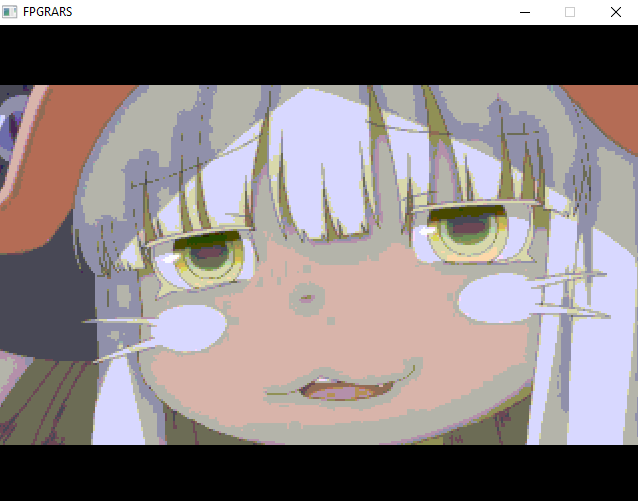
\includegraphics[width=8.47cm]{Nanachi_bmp}
            \label{fig:nanachi_bmp}
        \end{figure}
        %
        Infelizmente a sprite final fica com qualidade menor que a imagem original.
        Isso ocorre a princípio, devido ao modo como RGBs se tornam bytes de cor (assunto já detalhado): 
        tudo o mais constante, $R=100$ e $R=127$ geram a mesma cor no bitmap.
        
        \medskip
        
        Para contornar essa limitação na representação de cores, evite usar cores muito próximas como branco e azul muito claro, preto e vermelho escuro, etc.
        
        \medskip
        
        Com os conhecimentos adquiridos até aqui, não é difícil criar um programa que mostre no bitmap as 256 cores usadas pelo RARS.
        Uma forma de fazer isso é criar uma tile 16x16 cujo {\tt .data} é inteiramente um byte de cor, e variar esse byte até chegar no valor 256.
        
        \medskip
        
        A \autoref{fig:cores_do_rars} é um resultado desse algoritmo.
        Nela, a cor 0 está na quina superior esquerda, a cor 1 logo à sua direita, e por aí vai, até chegar ao fim do bitmap.
        
        \medskip
        
        Perceba que a cor 199 é a cor invisível e por isso apresenta a cor inicial da tela, o preto;
        note também que as cores voltam a se repetir após atingir o 256 (branco).
        %
        \begin{figure}[H]\centering
            \caption{
                Cores do RARS em ordem crescente. 
                O código executado para chegar a esta tela está presente no apêndice.}
            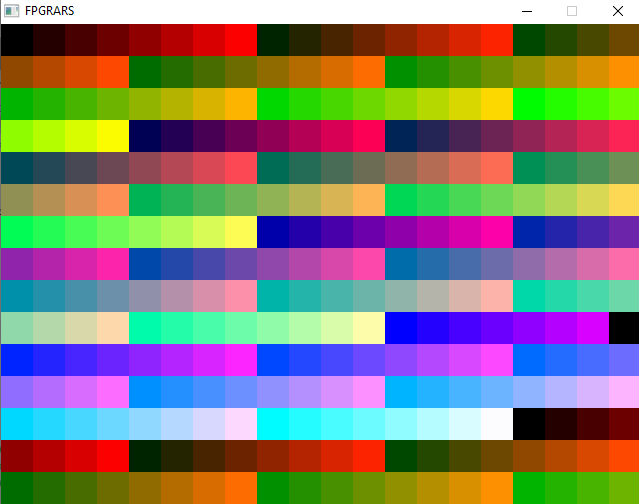
\includegraphics[width=8.47cm]{cores_do_rars}
            \label{fig:cores_do_rars}
        \end{figure}
        %
    %  
    
    
    \subsection{Curiosidade: como tornar uma cor cinza}
        Conhecido a fórmula de criação de bytes de cor, \autoref{eq:byte}, é simples arranjar a versão cinza de cada cor.
        Para tanto, sejam $(R,G,B)$ o RGB original e 
        $(R_c, G_c, B_c)$ 
        o RGB cinza associado.
        Então
        %
        \[
            R_c = G_c = B_c =
            \frac{R+G+B}{3}
        \]
        %
        e a obtenção do byte cinza é direta; basta seguir o fluxograma abaixo, por exemplo.
        %
        \begin{figure}[H]\centering
            \caption{%
                Fluxograma da lógica de acinzentar uma cor. $\beta_c$ é o valor (byte) da cor cinza associada a $R$, $G$, $B$.
                Este é o fluxograma que a função {\tt ByteCinza} segue.
            }
            \begin{tikzpicture}[>=latex', thick]
    \node [draw,
        minimum width=3.5em,
        minimum height=2em,
        rounded corners=5
    ] (inicio) at (0,0) {Início};
    
    \node [draw,
        minimum height=3.25em,
        right=1 of inicio
    ] (RGB) {
        \begin{minipage}{2cm}\centering
            Calcula\\
            $R$, $G$ e $B$
        \end{minipage}
    };
    
    \node [draw,
        minimum height=3.25em,
        right=1 of RGB
    ] (RGBc) {
        \begin{minipage}{2cm}\centering
            Obtém\\
            $R_c$, $G_c$ e $B_c$
        \end{minipage}
    };
    
    \node [draw,
        minimum height=3.25em,
        right=1 of RGBc
    ] (bytec) {
        \begin{minipage}{2cm}\centering
            Calcula $\beta_c$
        \end{minipage}
    };
    
    \node [draw,
        minimum width=3.5em,
        minimum height=2em,
        rounded corners=5,
        right=1 of bytec
    ] (fim) {Fim};
    
    % arrow heaven %
    \draw[->] (inicio) -- (RGB);
    \draw[->] (RGB) -- (RGBc);
    \draw[->] (RGBc) -- (bytec);
    \draw[->] (bytec) -- (fim);
\end{tikzpicture}
        \end{figure}
        %
        Na sequência, apresentam-se rotinas que juntas com a {\tt Print} realizam a impressão da versão cinza de uma sprite.
        Dito isso, é interessante que o leitor tome como exercício de fixação realizar a sua própria função {\tt ByteCinza}.
        %
        \lstinputlisting[
            language={[RISC-V]Assembler},
            caption={
                {\tt ByteCinza}, função que recebe um byte de cor em {\tt t5} e retorna a versão cinza desse byte também em {\tt t5}.
            }
        ]
        {ByteCinza.s}
        %
        \begin{remark}
            A pseudo instrução {\tt call} é uma versão mais poderosa da {\tt jal}, mas ela \textbf{também modifica {\tt t1}}.
            Por causa disso, da forma como a {\tt ByteCinza} foi feita, não podemos chamar a {\tt RGB2byte} via {\tt call}.
        \end{remark}
        %
        A {\tt byte2RGB} obtém a partir do byte de cor original os valores $R$, $G$, $B$ associados, e coloca-os em {\tt t0}, {\tt t1} e {\tt t2}, nessa ordem.
        Por outro lado, a {\tt RGB2byte} recebe o RGB em {\tt t0}, {\tt t1} e {\tt t2} e coloca o byte de cor associado em {\tt t5}.
        
        \medskip
        
        Confira essas rotinas a seguir.
        %
        \lstinputlisting[
            language={[RISC-V]Assembler},
            caption={
                {\tt byte2RGB}.
                Recebe um byte de cor em {\tt t5} e retorna seu RGB em {\tt t0}, {\tt t1}, {\tt t2}.
            }
        ]
        {byte2RGB.s}
        %
        \lstinputlisting[
            language={[RISC-V]Assembler},
            caption={
                {\tt RGB2byte}.
                Recebe um RGB em {\tt t0}, {\tt t1}, {\tt t2}, e retorna seu byte de cor em {\tt t5}.
            }
        ]
        {RGB2byte.s}
        %
        \begin{exercicio}
            Crie a função {\tt PrintCinza}, que consiste na
            modificação da {\tt Print} de forma que todo byte de cor (exceto o invisível) obtido do {\tt .data} em {\tt a0} seja impresso cinza no bitmap.
        \end{exercicio}
        %
        A seguir, apresentam-se alguns resultados da {\tt PrintCinza} definida no exercício acima.
        %
        \begin{figure}[H]\centering
            \caption
            {Sprites antes e depois da conversão para cinza.}
            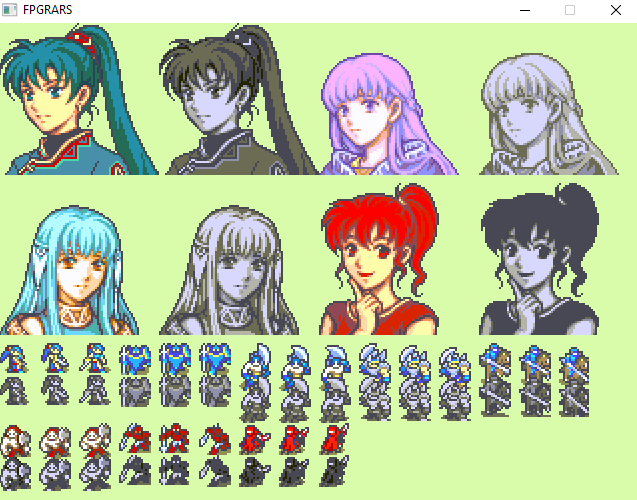
\includegraphics[width=0.8\textwidth]
            {grayscale}
        \end{figure}
        %
    
    \subsection{Criando animações no bitmap}
        Na Seção \ref{sec:frames} foi discutido uma maneira simples porém rudimentar de criar uma animação usando o bitmap.
        Agora, apresentaremos duas maneiras mais adequadas para o trabalho final:
        animação em intervalos regulares com sleep, e animação em intervalos distintos sem sleep.
        
        Por~``mais adequadas", entende-se funções inseridas num loop, que no caso do trabalho é o loop do jogo.
        Chamaremos esse loop de {\tt GameLoop}.
        %
        
        \subsubsection{Animação em intervalos regulares}
            Digamos que desejamos criar a animação \textit{idle} de um personagem de 3 poses diferentes.
            Por animação em intervalos regulares, entende-se que cada pose durará um certo tempo $t$ em ms.
            Neste contexto, é confortável usar a \ecall de sleep do RARS, que congela a execução do código por {\tt a0} milissegundos.
                
            \medskip
                
            Infelizmente, chamadas ao sistema não funcionam na FPGA, de forma que precisamos criar nossa própria função {\tt Sleep}, o que é tranquilamente satisfeito usando o registrado de status {\tt time}.
            Este registrador guarda a quantidade de ms despendida desde o início da execução do programa.
                
            \medskip
                
            Com isso em mente, é razoável pensar no seguinte fluxograma para a {\tt Sleep}.
            %
            \begin{figure}[H]\centering
                \caption{Lógica do {\tt Sleep}}
                \begin{tikzpicture}[>=latex', thick]
    \node [draw,
        minimum width=3.5em,
        minimum height=2em,
        rounded corners=5
    ] (inicio) at (0,0) {Início};
    
    \node [draw,
        minimum height=3.25em,
        right=1 of inicio
    ] (t0) {
        \begin{minipage}{2cm}\centering
            Registra o\\
            tempo atual,\\
            $t_0$
        \end{minipage}
    };
    
    \node [draw,
        minimum height=1em,
        right=1 of t0
    ] (t0+a0) {
        \begin{minipage}{2cm}\centering
            Calcula $t=t_0+t_\text{Sleep}$ 
        \end{minipage}
    };
    
    \node [draw,
        minimum height=1em,
        below=1 of t0+a0
    ] (t0') {
        \begin{minipage}{2cm}\centering
            Registra o tempo atual, $t_0'$ 
        \end{minipage}
    };
    
    \node [draw,
        diamond,
        minimum height=1em,
        right=1 of t0'
    ] (decisão) {
        \begin{minipage}{2cm}\centering
            $t_0'<t?$
        \end{minipage}
    };
    
    \node [draw,
        rounded corners=5,
        minimum width=2.5em,
        minimum height=2em,
        above=1 of decisão
    ] (fim) {Fim};
    
    % arrow hell
    \draw[->] (inicio) -- (t0);
    \draw[->] (t0) -- (t0+a0);
    \draw[->] (t0+a0) -- (t0');
    \draw[->] (t0') -- (decisão);
    \draw[->] (decisão) -- node [midway, fill=white, inner sep=1.5] {não$\,\,$} (fim);
    \draw[->] (decisão.south) --++ (0,-0.5) -| (t0'.south);
    \draw (decisão.south) ++ (0,-0.5) ++ (-1.75, 0)
    node [above] {sim$\,\,$};
\end{tikzpicture}
            \end{figure}
            %
            A partir da lógica exposta acima, ficamos com a seguinte função {\tt Sleep}.
            %
            \lstinputlisting[
                language={[RISC-V]Assembler},
                caption={Rotina de sleep compatível com a FPGA.}
            ]{Sleep.s}
            %
            \begin{remark}
                Economizaríamos um registrador, e duas instruções, se usássemos {\tt bltu} ao invés do {\tt sltu} e {\tt bne}.
                Infelizmente, por motivo desconhecido, essa versão do {\tt Sleep} não funciona no RARS.
            \end{remark}
            %
            \begin{exemplo}
                Executar o trecho abaixo {\tt Sleep} finaliza o programa após 10 segundos.
                %
                \begin{lstlisting}
                .text
                  li    a0, 10000
                  call  Sleep
                  li    a7, 10
                  ecall
                  
                  .include "Sleep.s"
                \end{lstlisting}
                %
                \begin{figure}[H]\centering
                    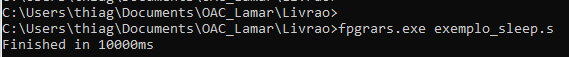
\includegraphics[width=\textwidth]
                    {exemplo_sleep10s}
                \end{figure}
            \end{exemplo}
            %
            Obtido o sleep, passamos à animação de fato.
            Lembre-se, queremos criar animação num contexto de loop, isto é, criar uma rotina {\tt Animacao} inserida num loop~``eterno"~como abaixo.
            %
            \begin{lstlisting}
            GameLoop:
              # ...
              call Animacao
              # ...
              j GameLoop
            \end{lstlisting}
            %
            Uma maneira de implementar a animação se inspira na máquina de estados finita: associamos a cada pose um estado, i. e., um número de 0 a 2, e imprimimos a pose de acordo com o estado.
            Por estética, é importante usar os frames de maneira inteligente, trocando para o próximo frame somente depois da sprite ser impressa lá. 
            Finalmente, antes da impressão de qualquer pose precisamos antes limpar aquele espaço.
            
            Por exemplo, limpar pode significar imprimir uma tile do mapa sobre o espaço desejado.
            Resumindo, nosso sistema de animação segue a seguinte ordem:
            %
            \begin{enumerate}
                \item [I.]
                chamada à função: 
                estado atual num frame (digamos, 0) com espaço livre no outro frame;
                
                \item [II.]
                armazenamento na pilha do espaço livre;
                
                \item [III.]
                \begin{enumerate}
                    \item [1.] atualiza o estado;
                    \item [2.] imprime, no outro frame, a pose de acordo com o estado;
                    \item [3.] troca o frame sendo exibido;
                \end{enumerate}
                
                \item [IV.]
                impressão da sprite armazenada na pilha (etapa II) sobre a pose no frame original (no caso, 0);
                
                \item [V.]
                retorno da função.
            \end{enumerate}
            
            \medskip
            
            O fluxograma e as figuras abaixo resumem e ilustram o discutido até aqui.
            %
            \begin{figure}[H]\centering
                \caption{Fluxograma da animação a ser executado em 1 laço do loop}
                \begin{tikzpicture}[>=latex', thick]
    \node [draw,
        minimum width=3.5em,
        minimum height=2em,
        rounded corners=5
    ] (inicio) at (0,0) {Início};
    
    \node [draw,
        minimum height=3.25em,
        right=1 of inicio
    ] (armazenamento) {
        \begin{minipage}{2.75cm}\centering
            Armazenamento
        \end{minipage}
    };
    
    \node [draw,
        minimum height=3.25em,
        below=1 of armazenamento
    ] (estados) {
        \begin{minipage}{1.5cm}\centering
            Atualiza\\
            estado
        \end{minipage}
    };
    
    \node [draw,
        minimum height=3.25em,
        right=1 of estados
    ] (pose) {
        \begin{minipage}{1.5cm}\centering
            Imprime\\
            pose
        \end{minipage}
    };
    
    \node [draw,
        minimum height=3.25em,
        right=1 of pose
    ] (frame) {
        \begin{minipage}{1.5cm}\centering
            Troca o\\
            frame
        \end{minipage}
    };
    
    \node [draw,
        minimum height=3.25em,
        above=1 of frame
    ] (recuperação) {
        \begin{minipage}{2cm}\centering
            Recuperação
        \end{minipage}
    };
    
    \node [draw,
        minimum width=3.5em,
        minimum height=2em,
        rounded corners=5,
        right=1 of recuperação
    ] (fim) {Fim};
    
    % arrow hell
    \draw [->] (inicio) -- (armazenamento);
    \draw [->] (armazenamento) -- (estados);
    \draw [->] (estados) -- (pose);
    \draw [->] (pose) -- (frame);
    \draw [->] (frame) -- (recuperação);
    \draw [->] (recuperação) -- (fim);
    
    % legendas de etapas (I, II, etc)
    \draw
        (-0.6, 0.6) node {\small I}
        (1.5, 0.8) node {\small II}
        (1.9, -1.4) node {\small III.1}
        (4.6, -1.4) node {\small III.2}
        (7.4, -1.4) node {\small III.3}
        (7.4, 0.8) node {\small IV}
        (10.7, .5) node {\small V}
    ;
    
\end{tikzpicture}
            \end{figure}
            %
            \begin{figure}[H]\centering
                \caption{
                    Ilustração da animação.
                    Os números arábicos indicam o frame, e os olhos indicam qual frame está sendo exibido.
                }
                \begin{tikzpicture}
    \draw [dashdotted]
        % etapa 1
        (0, 0) node {
\includegraphics{Lyn1}}
        (0, -1.5) node {
\includegraphics{fundo}}
        
        % etapa 2
        (2, 0) node {
\includegraphics{Lyn1}}
        (2, -1.5) node {
\includegraphics{fundo}}
        ++ (-0.5, 0.5) rectangle ++ (1, -1)
        
        % etapa 3
        (4, 0) node {
\includegraphics{Lyn1}}
        (4, -1.5) node {
\includegraphics{Lyn2}}
        
        % etapa 4
        (6, 0) node {
\includegraphics{fundo}}
        ++ (-0.5, 0.5) rectangle ++ (1, -1)
        (6, -1.5) node {
\includegraphics{Lyn2}}
        
        % etapa 5
        (8, 0) node {
\includegraphics{fundo}}
        (8, -1.5) node {
\includegraphics{Lyn2}}
    ;
    
    \def\eye{
              [fill=white]circle (0.2 and 0.1);
        \fill [gray!85] circle (0.1);
    }
    \draw
        % frames
        (-1, 0) node {\sf\textbf{0}}
        (-1.5, -0.75) --++ (10.5,0)
        (-1, -1.5) node {\sf\textbf{1}}
        
        % legendas
        (0, 0.5) node [above] {I}
        (2, 0.5) node [above] {II}
        (4, 0.5) node [above] {III}
        (6, 0.5) node [above] {IV}
        (8, 0.5) node [above] {V}
    ;
    
    % exibição do frame
    \def\eye{
        arc (30:150:0.2)
        arc (30:150:-0.2)
    }
    \def\pupil{
        circle (0.09)
    }
    \draw
        (0.7, .55) \eye
        (2.7, .55) \eye
        (4.7, -0.95) \eye
        (6.7, -0.95) \eye
        (8.7, -0.95) \eye
    ;
    \fill
        (0.53, .55) \pupil
        (2.53, .55) \pupil
        (4.53, -0.95) \pupil
        (6.53, -0.95) \pupil
        (8.53, -0.95) \pupil
    ;
    
    % descrições
    \draw
        (0, -2.5) node {\small\sf
            \begin{minipage}{2cm}\centering
                Função é\\
                chamada
            \end{minipage}
        }
        
        (2, -2.5) node {\small\sf
            \begin{minipage}{2cm}\centering
                Guarda\\
                o fundo
            \end{minipage}
        }
        
        (4, -2.5) node {\small\sf
            \begin{minipage}{2cm}\centering
                Atualiza pose,\\
                troca o frame
            \end{minipage}
        }
        
        (6, -2.5) node {\small\sf
            \begin{minipage}{2cm}\centering
                Imprime\\
                o fundo
            \end{minipage}
        }
        
        (8, -2.5) node {\small\sf
            \begin{minipage}{2cm}\centering
                Retorna
            \end{minipage}
        }
    ;
    
\end{tikzpicture}
            \end{figure}
            %
            Tendo em vista o apresentado acima, faz sentido compor o {\tt Animacao}, principalmente, por 3 funções, cujos nomes deixam claro objetivos:
            {\tt GuardaFundo},
            {\tt AtualizaPose} e
            {\tt ImprimeFundo}. 
            
            \medskip
            
            Para que a animação funcione adequadamente, (i) precisamos saber qual frame está sendo exibido; (ii) criaremos ainda uma label {\tt personagem} que guarda a posição $(x,y)$ do fundo/pose no bitmap e o estado daquele personagem.
            Com isso dito, definimos com as seguintes tabelas de argumentos.
            %
            \begin{table}[H]\centering
                \caption{Argumentos da {\tt Animação}}
                \begin{tabular}{cc}
                    \toprule
                    Registrador & Conteúdo \\
                    \midrule\midrule
                    {\tt s0} & frame atual \\
                    {\tt a0} & label do personagem \\
                    \bottomrule
                \end{tabular}
            \end{table}
            %
            \begin{table}[H]\centering
                \caption{Argumentos da {\tt GuardaFundo}, {\tt ImprimeFundo}, {\tt AtualizaPose}}
                \begin{tabular}{cc}
                    \toprule
                    Registrador & Conteúdo \\
                    \midrule\midrule
                    {\tt s0} & frame atual \\
                    {\tt a1} & $x$ do personagem \\
                    {\tt a2} & $y$ do personagem \\
                    {\tt a3} & estado do personagem \\
                    \bottomrule
                \end{tabular}
            \end{table}
            %
            Como estamos trabalhando com mudança de poses em intervalos iguais e usando sleep, {\tt AtualizaPose} sempre colocará o estado atual como estado anterior + 1 mod 3 quando for chamada;
            daí, o estado 0 vai para 1, 1 vai para 2, e 2 vai para 0.
            
            Uma maneira de escrever essa rotina é mostrada abaixo.
            %
            \lstinputlisting[
                language={[RISC-V]Assembler}, 
                caption={
                    Função {\tt AtualizaPose}, reponsável por implementar toda a etapa III da animação.
                }
            ]{AtualizaPose.s}
            %
            Quanto ao {\tt GuardaFundo} e {\tt ImprimeFundo}, podemos nos basear na {\tt Print}, apenas usando a pilha no lugar do bitmap/{\tt a0}, respectivamente.
            Outra diferença é que aqui vamos assumir largura e altura da sprite de fundo fixas e iguais a 16, para simplificar o código.
            
            Confira uma possível implementação do {\tt GuardaFundo} abaixo.
            %
            \lstinputlisting[
                language={[RISC-V]Assembler},
                caption={
                    Função {\tt GuardaFundo}. 
                    Note como o fundo é armazenado na pilha
                }
            ]{GuardaFundo.s}
            %
            Dada a implementação acima, se a {\tt ImprimeFundo} simplesmente tirasse os bytes da pilha a partir da posição onde o {\tt GuardaFundo} a deixou, a sprite do fundo sairia ``de trás pra frente"~no bitmap.
            Por causa disso, vamos usar o registrador {\tt t6} para ajustar a pilha quando necessário no {\tt ImprimeFundo}, veja o próximo listing (e compare-o com o do {\tt GuardaFundo}).
            %
            \lstinputlisting[
                language={[RISC-V]Assembler},
                caption={
                    Função {\tt ImprimeFundo}. 
                }
            ]{ImprimeFundo.s}
            %
            \begin{exercicio}
                Modifique a {\tt GuardaFundo} e {\tt ImprimeFundo} apresentadas acima para lidarem com um fundo de dimensões {\tt a4}x{\tt a5} ao invés de 16x16. 
            \end{exercicio}
            %
            Finalmente, obtemos o seguinte para a {\tt Animacao}, 
            %
            \lstinputlisting[
                language={[RISC-V]Assembler},
                caption={Função {\tt Animacao}}
            ]{Animacao.s}
            %
            que foi projetado para ser chamado num loop como o abaixo.
            %
            \lstinputlisting[
                language={[RISC-V]Assembler},
                caption={
                    Inicialização e {\tt GameLoop}.
                    {\tt Sleep} é a mesma função do início desta subseção.
            }
            ]{GameLoop.s}
            %
            Rodando o programa no RARS e no FPGRARS, vê-se que a animação é executada corretamente, com exceção do já comentado mau comportamento do RARS com a cor invisível. 
            
            Uma vantagem do método de animação que fizemos aqui é a facilidade com que ela pode ser estendida para múltiplos personagens: 
            bastaria introduzir as devidas labels e criar um {\tt AtualizaPose} para cada personagem/objeto (assim como atualizar o frame exibido fora do {\tt AtualizaPose}).
            
            Entretanto, um potencial ponto ruim do método é o uso do sleep, que pode vir a tornar o jogo ``cortado"~e insensível aos inputs do usuário.
            Além disso, animações com movimentos abruptos não são bem implementadas por esse método.
            
            Por causa disso, na sequência apresentamos um estilo de animação que não usa o sleep e portanto não trava o sistema e comporta movimentos bruscos, que nomeamos ``animação por intervalos distintos".
            %
        %
        
        \subsubsection{Animação em intervalos distintos}
            Digamos que desejamos fazer a seguinte animação abaixo, onde a pose do meio dura bem menos que as outras duas poses.
            %
            \begin{figure}[H]\centering
                \caption{Sprites a serem animadas e suas durações}
                \begin{subfigure}{0.32\textwidth}
                    \centering
                    \caption{{\tt Assassin1} - 1000 ms}
                    
\includegraphics{Assassin1}
                \end{subfigure}
                \begin{subfigure}{0.32\textwidth}
                    \centering
                    \caption{{\tt Assassin2} - 50 ms}
                    
\includegraphics{Assassin2}
                \end{subfigure}
                \begin{subfigure}{0.32\textwidth}
                    \centering
                    \caption{{\tt Assassin3} - 300 ms}
                    
\includegraphics{Assassin3}
                \end{subfigure}
            \end{figure}
            %
            Em comparação com a lógica da animação anterior, o que precisamos fazer aqui é apenas mudar como os estados são atualizados -- {\tt GuardaFundo} e {\tt ImprimeFundo} continuarão as mesmas, e a ilustração e o fluxograma continuam válidos.
            
            Para tanto, antes de mais nada, é importante fixar as sequências da animação, o que fazemos pelo diagrama abaixo, inspirado numa MEF.
            %
            \begin{figure}[H]\centering
                \caption{Sequência de estados da animação com intervalos distintos.}
                \begin{tikzpicture}[> = latex']
    \node [draw, ultra thick,
        circle,
        radius=1
    ] (0) at (0,0) {0};
    
    \node [draw, ultra thick,
        circle,
        radius=1,
        below right=1 of 0
    ] (2) {2};
    
    \node [draw, ultra thick,
        circle,
        radius=1,
        above right=1 of 2
    ] (1) {1};
    
    % legendas
    \draw
        (0) ++ (0, 0.5) node [anchor=south] {
            \begin{minipage}{2cm}\centering
                1000 ms\\
                \tt Assassin1
            \end{minipage}
        }
        
        (1) ++ (0, 0.5) node [anchor=south] {
            \begin{minipage}{2cm}\centering
                50 ms\\
                \tt Assassin2
            \end{minipage}
        }
        
        (2) ++ (0,-0.5) node [anchor=north] {
            \begin{minipage}{2cm}\centering
                300 ms\\
                \tt Assassin3
            \end{minipage}
        }
    ;
    
    % arrow hell
    \draw [->] (0) -- (1);
    \draw [->] (1) -- (2);
    \draw [->] (2) -- (0);
\end{tikzpicture}
            \end{figure}
            %
            Para que o novo sistema funcione, criaremos 4 labels:
            uma, {\tt changeTime}, que guarda o tempo do sistema de quando uma nova pose foi atingida, e três, {\tt animTimeX}, que guardam o tempo em ms que cada pose {\tt X} deve permanecer na tela.
            
            \medskip
            
            Esses valores serão usados pelo módulo {\tt AtualizaEstados}, que será chamado no início da {\tt AtualizaPose}.
            Essa função deve, para cada estado, verificar se a pose atual deve ou não ser trocada para daí atualizar o estado (em caso afirmativo) ou não (em caso negativo). 
            Trata-se de uma rotina que tem {\tt a3}, o estado atual, tanto como input como output.
            
            Sendo a lógica da função simples e similar ao da {\tt Sleep}, mostramos imediatamente sua implementação sem apresentar o fluxograma.
            %
            \lstinputlisting[
                language={[RISC-V]Assembler},
                caption={Função {\tt AtualizaEstados}}
            ]
            {AtualizaEstados.s}
            %
            Realizando as adaptações de label necessárias na {\tt AtualizaPose} (basicamente, trocar {\tt Lyn} por {\tt Assassin}), o novo loop de jogo a seguir nos dá a animação desejada%
            \footnote{%
                Repare que foi preciso ainda aumentar a área da limpeza para uma tile 20x20.
            }.
            %
            \lstinputlisting
            [
                language={[RISC-V]Assembler},
                caption={{\tt NewGameLoop}, feito para a animação sem sleep.}
            ]
            {NovoGameLoop.s}
        %
        A listing acima encerra o tópico de animações.
        Em geral, nos jogos de OAC, essas animações são frequentemente ligadas a algum input usuário; por exemplo, a pressionar a tecla d move o personagem para a direita.
        
        Dessa forma, continuaremos o texto explicando como processar inputs do usuário, isto é, teclas pressionadas no teclado KDMMIO.
        %
    %
    % \subsection{Analisando o system: o {\ttfamily printChar}}
    % \subsection{Resumo da seção}
  
  \section{O teclado KDMMIO}
    \subsection{Leitura por keypoll}
    \subsection{Leitura por interrupção}
    \subsection{Integração teclado-animação}
    % \subsection{Resumo da seção}

  \section{Como tocar música no RARS/FPGRARS}
    \subsection{Como tocar uma nota: as \ecall's de midi}
    \subsection{Tocando música dentro de um loop de nota em nota}
    \subsection{Analisando o system: {\ttfamily midiOut}}
    % \subsection{Resumo da seção}
  
  \section{Apêndice}
    \subsection{Cores do RARS}
        \lstinputlisting[language={[RISC-V]Assembler}]
        {cores_do_RARS.s}
\end{document}
